\documentclass[fr]{../../../../../../eplexam}

\hypertitle{Théorie des graphes (MAJ)}{5}{INMA}{1961}{2014}{Janvier}
{Etudiants MAP de 2017}
{Vincent Blondel et Jean-Charles Delvenne}

\section{}

Le Père Noël, perché sur les toits de la ville enneigée, est embarrassé: sa hotte contient bien un iguanodon, une jument verte, un kangourou, un lapin rose, un mouton, un nasique, un ours et un phoque, mais ses lutins ont oublié de noter sur chaque cadeau le nom de son destinataire. Heureusement, il connaît bien le coeur des enfants et sait par exemple que le petit Guillaume aime les dinosaures. Les goûts de chacun sont synthétisés dans le graphe ci-dessous.

Le père Noël peut-il attribuer un jouet à Alphonse, Bérengère, Charlotte, Désiré, Etienne, Firmin, Guillaume et Henri et ne faire que des heureux? Sinon, comment briser le moins de coeurs possible? Justifiez vos affirmations.
\begin{figure}[h!]
	\centering
	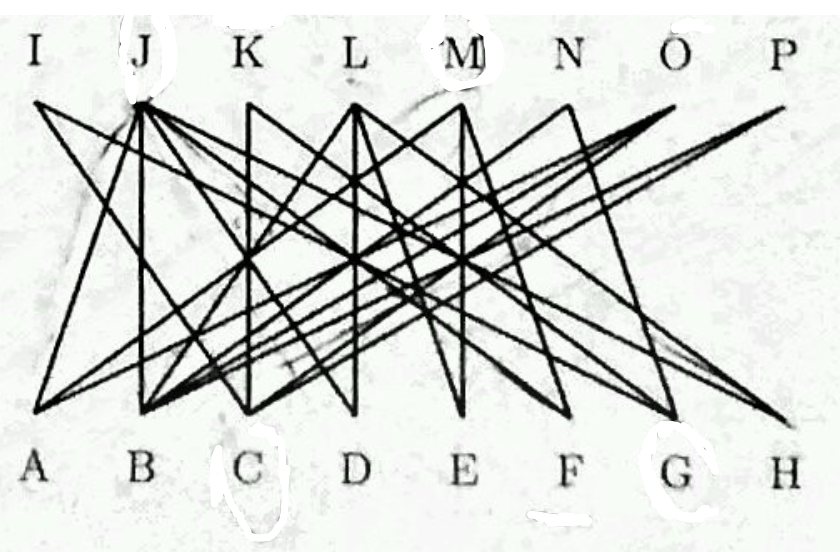
\includegraphics[scale=0.5]{juin2014MajQ1.PNG}
	\caption{Graphe de la question 1}
\end{figure}

\begin{solution}
	
Nous pouvons remarquer qu'il n'est pas possible de satisfaire tous les enfants. En effet, I,K,N et P sont uniquement reliés à B,C et G. 
Un couplage maximum peut être : \{(N,G),(I,C),(P,B),(J,D),(L,E),(M,F),(O,A)\}
	
\end{solution}
	
\section{}

Démontrez que :

\begin{enumerate}
	\item tout graphe planaire simple biparti à n noeuds a au plus 2n - 4 arêtes.
	
	\item le graphe biparti complet à 3+3 noeuds n'est pas planaire.
	
\end{enumerate}

Indice : la formule d'Euler s'énonce: $f + n = 2 + e$.

\begin{solution}

\begin{enumerate}
	\item Par l'absurde : on peut avoir $2n-4+1$ arêtes. Nous avons la formule d'Euler et la relation $3f \leq 2e$. Nous trouvons donc que $n \leq 3$ et donc nous pouvons faire un graphe simple biparti de 3 noeuds avec ($2\cdot3-3 $) 3 arêtes, c'est impossible, il y a donc une contradiction.
	
	\item $n = 6$ et $e = 9$. Nous pouvons utiliser ce qui est dit dans la 1e  sous-question et remarquer qu'ici $2n - 4 = 8 < 9$ et donc le graphe ne peut être planaire.
	
\end{enumerate}
	
\end{solution}

\section{}

Démontrez que G est un arbre (c'est-à-dire un graphe simple connexe et sans cycle) ssi G est connexe et supprimer toute arête déconnecte G. \\

\begin{solution}
	
Dans le sens $\Rightarrow$. Raisonnons par l'absurde et supposons le temps d'un instant qu'il existe une arête $e$  dans $G$ qui ne déconnecte pas $G$. Notons $v_1$ et $v_2$ les sommets adjacents à cette arête. Par hypothèse absurde, si nous l'ôtons, il existera un chemin $\mathcal C$ de $v_1$ à $v_2$ car le graphe reste connexe. Remettons l'arête $e$. Il existe donc un cycle composé de $\mathcal C$ et l'arête $e$. Ce qui est absurde puisque nous avions supposé le graphe être un arbre.

Dans le sens $\Leftarrow$. Considérons un graphe $G$ connexe et tel que toute arête ôtée le déconnecte à jamais. Supposons, par l'absurde, qu'il possède un cycle $\mathcal C$ et soit $v$ une arête de ce cycle. Notons $e_1$,$e_2$ les sommets adjacents à cette arête. Si on ôte $v$, $e_1$ et $e_2$ sont encore connectés car dans un cycle. La proposition suit \emph{ad reductio absurdum}.

\end{solution}


\section{}
Soit $\chi$ le nombre chromatique d'un graphe simple à $n$ noeuds (c'est-à-dire le plus petit nombre de couleurs d'un coloriage propre des noeuds), et $\alpha$ la plus grande taille d'un ensemble indépendant (c'est-à-dire l'ensemble de noeuds non-adacents deux à deux).

\begin{enumerate}
	\item Calculez ces nombres pour 
	\begin{itemize}
		\item le graphe biparti complet à $n$ noeuds,
		\item le cycle à $n$ noeuds,
		\item la roue à $n$ noeuds (\url{https://fr.wikipedia.org/wiki/Graphe_roue}),
		\item l'arbre binaire complet à $k$ niveaux et donc à $2^k -1$ noeuds.
	\end{itemize}
	
	\item Démontrez que $\chi +\alpha \leq n + 1$.
	
	\item Donnez une famille infinie de graphes qui vérifie cette borne avec égalité.
	
\end{enumerate}

\begin{solution}

\begin{enumerate}

\item \begin{itemize}
	\item $\chi = 2 $ et $\alpha$ est égal au plus grand des 2 nombres de la bipartition ($n/2$ si les 2 font la même taille, $n$ si les 2 ensembles sont de taille $n$ ?).
	\item $\chi = 2$ si $n$ est pair, 3 sinon. Et $\alpha = n/2 $ si $n$ pair, $(n-1)/2$ sinon.
	\item $\chi = 3$ si $n$ est impair, 4 sinon. Et $\alpha = n/2 - 1 $ si $n$ est pair, $(n-1)/2$ sinon.
	\item $\chi =2$ et $\alpha = \sum_{i = 0}^{k/2} 2(k-1-2i)$.
\end{itemize}

\item Par induction sur $n$ : si $n=1$ alors $$\chi=1,\alpha=1 \Rightarrow \chi+\alpha\leq n+1=2$$
On suppose la propriété vraie pour un graphe à $n-1$ noeuds, si on retire un noeud à un graphe de taille $n$, on identifie son ensemble indépendant et son nombre chromatique. On remet ensuite le noeud :
\begin{itemize}
	\item Soit on peut colorier le noeud dans une couleur déjà existante alors $\chi$ est inchangé et il peut potentiellement être inclus dans le plus grand ensemble indépendant, auquel cas $\alpha_n=\alpha_{n-1}+1$ et la propriété est toujours vérifiée.
	\item Soit on doit utiliser une nouvelle couleur $\Rightarrow \chi_{n} = \chi_{n-1}+1$ et dans ce cas, le noeud ne peut être inclus dans l'ensemble indépendant le plus grand (sinon on aurait pu le colorier dans la couleur de celui-ci). Donc $\alpha_n=\alpha_{n-1}$.
\end{itemize}

 \paragraph{Alternative} Soit G, un coloriage propre du graphe serait de colorier tout les noeuds du plus grand ensemble indépendant (de taille $\alpha$) en une même couleur et de colorier les $n-\alpha$ noeuds restants en $n-\alpha$ couleurs. Le coloriage propre obtenu comporte alors $n-\alpha+1$ couleurs. On a donc $\chi \leq n-\alpha+1$ ou encore $\chi + \alpha \leq n+1$.

\item L'ensemble des graphes complets $K_n : \chi=n$, $\alpha=1 \Rightarrow \chi+\alpha=n+1$

\end{enumerate}

\end{solution}

\section{}

Nous vous proposons de changer les règles de la coupe du monde de football. Chaque groupe contient $k$ équipes. Lors d'un mach entre équipes d'un même groupe, le gagnant remporte deux points, et lors d'un match nul, les deux équipes remportent chacun un point. Supposons également que seul le premier du groupe soit qualifié pour la suite du tournoi (en cas d'égalité, c'est celui qui a marqué le plus de buts qui gagne). Supposons enfin que l'équipe $i$ a pour l'instant $u_i$ points et qu'il reste $r_{ij}$ matches à jouer entre les équipes $i$ et $j$.

\begin{enumerate}
	\item On cherche à décider si la Belgique est \textit{mathématiquement éliminée}, selon l'expression consacrée des commentateurs sportifs. Un algorithme de force brute consiste à examiner tous les déroulements possibles de tous les matches restants et à examiner si dans chacun d'entre eux la Belgique est éliminée. Quelle est la complexité temporelle de cet algorithme, en notation $\mathcal{O}(\cdot)$? Est-ce un algorithme efficace, c'est-à-dire de complexité polynomiale en la taille des données?
	
	\item Réduisez la question ci-dessus à un problème de flot dans un graphe. Cela veut dire qu'il faut pouvoir répondre à la question de l'élimination mathématique en résolvant un problème de flot, et en regardant si le flot trouvé possède une propriété particulière. Pour cela, un bon point de départ est de voir la réserve de points comme la source et les différentes équipes du groupe H (celui de la Belgique) comme les destinations (ou puits).
	
	\item Le problème de l'élimination mathématique est-il dans $\mathcal P$?
	
	\item Bonus: comment traiter le cas où les deux premiers du groupe sont qualifiés?
	
\end{enumerate}

\begin{solution}
	
	\begin{enumerate}
		
		\item Etant donné qu'il y a 3 résultats possibles (gagné, nul, perdu), il faut analyser les 3 cas pour tous les matches restant dans la poule H (celle de la Belgique). On a donc un algorithme en $\mathcal{O}(3^{\Sigma_{i,j=1}^{k} r_{ij}}) , i \neq j$ , ce qui n'est pas du tout efficace vu que c'est exponentiel et non polynomial.
		
		\item Pour réduire la question en termes de flots, on met une source  \emph{infinie} de points d'un côté et les équipes (les noeuds, il y en a $k$) de l'autre. Au centre, en colonne, on met des noeuds représentant les matches à jouer. On relie la source à chaque match avec une arête de capacité deux. De même, on relie chaque match au deux équipes participantes. Une équipe peut être reliée plusieurs fois. On calcule le flot max pour chacune des équipes de $1$ à $k$. Avec la valeur du flot, on additionne les points que l'équipe avait déjà. Si $f_i$ est le flot de la $i$-eme team, alors on fait $u_i + f_i$. Si $u_b + f_b$ ($b$ pour Belgique) est max, on conclut que la Belgique peut gagner Sinon, elle peut rentrer au pays.
		
		\item Oui, il est dans $\mathcal P$. En effet pour calculer le flot, il existe un algorithme polynomial (Ford Fulkerson,...) et ici on fait $k- 1$ appels à un algo polynomial.
		
		\item Même idée, mais on regarde si la belgique est deuxieme ou première.
		
	\end{enumerate}
	
\end{solution}

\end{document}
